\newlength\imagewidth
\newlength\imagescale
\pgfmathsetlength{\imagewidth}{0.3\linewidth}
\pgfmathsetlength{\imagescale}{\imagewidth/128}
\tikzsetnextfilename{mr_k_space}
\begin{tikzpicture}[x=\imagescale,y=-\imagescale]
	\node[anchor=north west,inner sep=0pt,outer sep=0pt] (ksp) at (-0.5,-0.5)
   {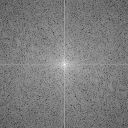
\includegraphics[width=\imagewidth]{images/kspace}};
	\draw[thick,->] (-4, 64) -- (131, 64) node [right] {$k_x$};
	\draw[thick,->] (64, 131) -- (64, -4) node [above] {$k_y$};
	\filldraw (64, 54) coordinate (ksp1) circle (1.5pt);
	\filldraw (69, 64) coordinate (ksp2) circle (1.5pt);
	\filldraw (60, 56) coordinate (ksp3) circle (1.5pt);
	\filldraw (54, 79) coordinate (ksp4) circle (1.5pt);
	
	\node[anchor=north west,inner sep=0pt,outer sep=0pt] (kspf1) at ($(ksp.north east) + (1cm, 0)$) {
\includegraphics[width=.1509\linewidth]{images/spatialfreq_0_10}};
	\draw[->, shorten >=1mm] (ksp1) -- (kspf1.west);
	\node[anchor=south west,inner sep=0pt,outer sep=0pt] (kspf2) at ($(ksp.south east) + (1cm, 0)$) {
\includegraphics[width=.1509\linewidth]{images/spatialfreq_5_0}};
	\draw[->, shorten >=1mm] (ksp2) -- (kspf2.west);
	\node[anchor=north east,inner sep=0pt,outer sep=0pt] (kspf3) at ($(ksp.north west) - (1cm, 0)$) {\reflectbox{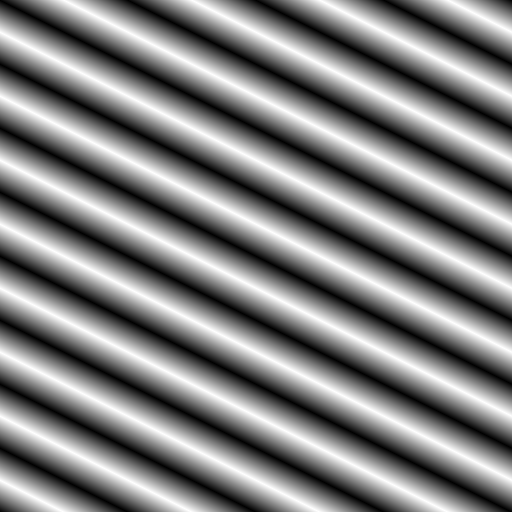
\includegraphics[width=.1509\linewidth]{images/spatialfreq_-4_8}}};
	\draw[->, shorten >=1mm] (ksp3) -- (kspf3.east);
	\node[anchor=south east,inner sep=0pt,outer sep=0pt] (kspf4) at ($(ksp.south west) - (1cm, 0)$) {\reflectbox{
\includegraphics[width=.1509\linewidth]{images/spatialfreq_-10_-15}}};
	\draw[->, shorten >=1mm] (ksp4) -- (kspf4.east);
\end{tikzpicture}
